\section{Theory}
\subsection{Det här är också en underrubrik}
\subsubsection{Det här är underrubrikens rubrik}
In today's automotive companies huge resources are put in optimising and developing efficient processes that are in favour of the environmental, safety on the roads and antonyms cars. In this cluster of new technology is something called "V2V" \textit{(Vehicle-to-vehicle communication)}. V2V is a wireless transmission system between cars on the road. The reason and idea behind this technology is to get cars around each other to communicate with each other to reduce the risk of both collision and more energy effective driving. The information that is sent between the cars are their speed, position and direction.

\begin{figure}[H]
    \centering
    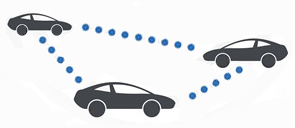
\includegraphics{images/V2VLan.png}
    \caption{LAN network}
\end{figure}
This information is sent over an AD-HOC [reference] network. AD-HOC is a local area network (LAN) that's used in close area networking. This is used instead of a global network “cloud network”. 
\begin{figure}[H]
    \centering
    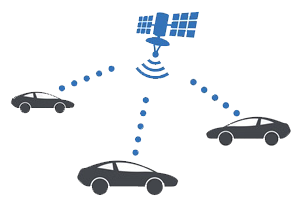
\includegraphics{images/V2VGlobal.png}
    \caption{Cloud network}
\end{figure}


AD-HOC is used for many reasons but mostly because a global network can have delay between the server and the cars and is hard to use in areas with bad connection to the grid. By using AD-HOC the delay in the signals between the vehicles are reduced and in traffic a shorter delay can save lives.
\bigskip

The goal of V2V is to reduce the total of cars crashes and especially in the future when cars are becoming completely autonomous and driving by themselves. This is where the V2X project enters the picture, \textit{"Because if cars are to communicate with each other, why not let the cars communicate with everything on the road like bikes, traffic lights and pedestrian crossings. Is that possible?"} It had reduced the risk of collision even more.
\bigskip

The technology used is called "Cooperative Intelligent Transport Systems" (C-ITS).  “ITS-G5” is a broadcast technology based on an evolution of the wireless standard 802.11p. It is the only validated and available technology on the market and capable of delivering secure AD-HOC direct vehicle-to-vehicle and/or vehicle-to-infrastructure communication. ITS-G5 is running in the designated 5.9 GHz frequency band that is foreseen for road safety. We emphasise that all technologies that run in this frequency band should not cause interference with each other and be interoperable.C-ITS should be able to demonstrate its capability to co-exist with electronic road charging, the enforcement of drive and rest times and weights and dimensions on the adjacent 5.8 GHz frequency band. [reference]
